\documentclass{standalone}
\usepackage{steinmetz}
\usepackage{tikz}
\begin{document}
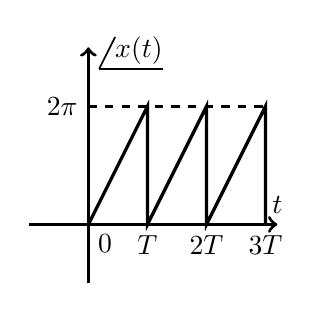
\begin{tikzpicture}[scale=1.5]
    \draw[->,very thick](2,0)--(4.1,0)node[above]{$t$};
    \draw[->,very thick](2.5,-0.5)--(2.5,1.5)node[right]{$\phase{x(t)}$};
    \draw[dashed,very thick](2.5,1)node[left]{$2\pi$}--(4,1);
    \node[below right]at(2.5,0){$0$};
    \draw[-,very thick](2.5,0)--(3,1)--(3,0)node[below]{$T$}--(3.5,1)--(3.5,0)node[below]{$2T$}--(4,1)--(4,0)node[below]{$3T$};
\end{tikzpicture}
\end{document}